% ============================================================
%  SCHOLA DOMESTICA — Magister Mathematica
%  Level 1 | Week 10 | Day 1
%  Topic: Addition Facts — +4 and +5, Sums to 8
% ============================================================
\documentclass[12pt, letterpaper]{article}

\usepackage[top=1in, bottom=1in, left=1in, right=1in]{geometry}
\usepackage[T1]{fontenc}
\usepackage[utf8]{inputenc}
\usepackage{lmodern}
\usepackage{microtype}
\usepackage{amsmath}
\usepackage{xcolor}
\usepackage{tikz}
\usepackage{array}
\usepackage{enumitem}
\usepackage{multicol}
\usepackage{mdframed}
\usepackage{fancyhdr}

\definecolor{scholared}{RGB}{160,30,30}
\definecolor{scholagold}{RGB}{180,140,40}
\definecolor{scholacream}{RGB}{253,248,235}
\definecolor{scholagreen}{RGB}{50,110,60}
\definecolor{scholablue}{RGB}{40,80,140}

\pagestyle{fancy}
\fancyhf{}
\renewcommand{\headrulewidth}{0.6pt}
\fancyhead[L]{\small\textcolor{scholared}{\textbf{Schola Domestica — Magister Mathematica}}}
\fancyhead[R]{\small\textcolor{scholared}{Level 1 · Week 10 · Day 1}}
\fancyfoot[C]{\small\textcolor{gray}{— \thepage\ —}}

\newcommand{\answerline}{\underline{\hspace{2.5cm}}}
\newcommand{\biganswerline}{\underline{\hspace{4cm}}}
\newcommand{\numbox}{\tikz{\draw[scholablue,thick](0,0)rectangle(1.2cm,0.85cm);}}

\newmdenv[
  backgroundcolor=scholacream,
  linecolor=scholared,
  linewidth=1.5pt,
  roundcorner=6pt,
  innertopmargin=8pt,
  innerbottommargin=8pt,
  innerleftmargin=10pt,
  innerrightmargin=10pt
]{lessonbox}

\newmdenv[
  backgroundcolor={rgb,255:red,235;green,245;blue,235},
  linecolor=scholagreen,
  linewidth=1.2pt,
  roundcorner=4pt,
  innertopmargin=6pt,
  innerbottommargin=6pt,
  innerleftmargin=8pt,
  innerrightmargin=8pt
]{enrichbox}

\begin{document}

\begin{center}
  {\LARGE\textbf{\textcolor{scholared}{Addition Facts:}}}\\[4pt]
  {\Large\textcolor{scholagold}{\textit{Adding Four and Adding Five}}}\\[6pt]
  {\small Name: \biganswerline \hspace{1cm} Date: \answerline}
\end{center}

\vspace{4pt}
\noindent\textcolor{scholared}{\rule{\linewidth}{1pt}}
\vspace{4pt}

% IMAGE PROMPT (Beatrix Potter watercolour style):
% Five small field mice sit in a row on a log, each holding a bluebell. Four more mice arrive from
% the right. Soft dappled forest light, blue and green palette, white paper background, no text.

\begin{lessonbox}
\textbf{Adding larger numbers — count on from the bigger part.}\\[6pt]
\begin{itemize}[leftmargin=1.5em, itemsep=3pt]
  \item \textbf{$+4$}: start at the bigger number, count on 4.\\
    \hspace{1em} $3 + 4$: start at \textit{four} (bigger) … 5, 6, \textbf{7}
  \item \textbf{$+5$}: start at the bigger number, count on 5 (or use your whole hand!).\\
    \hspace{1em} $2 + 5$: start at \textit{five} … 6, 7, \textbf{7} \quad [\textit{hold up 5 fingers, count on 2 more}]
\end{itemize}
\medskip
\noindent\textbf{Tip:} Always start counting from the \emph{larger} addend — it is faster!
\end{lessonbox}

\bigskip

% ===== PART I: +4 on number line =====
\noindent\textcolor{scholared}{\large\textbf{Part I — Adding Four}} \hfill \textit{(Problems 1–5)}

\medskip
\noindent\textit{Hop 4 spaces on the number line. Write the sum.}

\bigskip

% Number line 0–9
\noindent
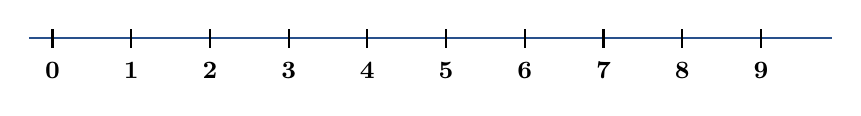
\begin{tikzpicture}
  \draw[thick, scholablue] (0,0) -- (10.2,0);
  \foreach \n in {0,...,9} {
    \draw[thick] (\n*1.0+0.3, -0.12) -- (\n*1.0+0.3, 0.12);
    \node[below] at (\n*1.0+0.3, -0.18) {\small\textbf{\n}};
  }
\end{tikzpicture}

\bigskip

\noindent
\begin{tabular}{@{}p{7.0cm} p{7.0cm}@{}}
\textbf{1.}\; Start at 0, hop 4: $0 + 4 =$ \numbox &
\textbf{2.}\; Start at 1, hop 4: $1 + 4 =$ \numbox \\[12pt]
\textbf{3.}\; Start at 2, hop 4: $2 + 4 =$ \numbox &
\textbf{4.}\; Start at 3, hop 4: $3 + 4 =$ \numbox \\[12pt]
\multicolumn{2}{@{}l@{}}{\textbf{5.}\; Start at 4, hop 4: $4 + 4 =$ \numbox \quad \textit{(this is a doubles fact!)}}
\end{tabular}

\bigskip\bigskip

% ===== PART II: +5 with dots =====
\noindent\textcolor{scholared}{\large\textbf{Part II — Adding Five}} \hfill \textit{(Problems 6–10)}

\medskip
\noindent\textit{The five-dot row shows one part. Count on from 5. Write the sum.}

\bigskip

% Five-frame visual for +5 facts
\noindent
\begin{tabular}{@{}p{7.0cm} p{7.0cm}@{}}

% Problem 6: 1+5=6
\textbf{6.}

\begin{tikzpicture}[baseline=-0.5ex]
  \foreach \i in {1,...,5} { \filldraw[scholablue] (\i*0.38,0) circle (0.13cm); }
  \filldraw[scholagold] (5*0.38+0.5,0) circle (0.13cm);
\end{tikzpicture}
\; $1 + 5 =$ \numbox
&
% Problem 7: 2+5=7
\textbf{7.}

\begin{tikzpicture}[baseline=-0.5ex]
  \foreach \i in {1,...,5} { \filldraw[scholablue] (\i*0.38,0) circle (0.13cm); }
  \foreach \i in {1,2} { \filldraw[scholagold] (5*0.38+\i*0.4,0) circle (0.13cm); }
\end{tikzpicture}
\; $2 + 5 =$ \numbox \\[18pt]

% Problem 8: 3+5=8
\textbf{8.}

\begin{tikzpicture}[baseline=-0.5ex]
  \foreach \i in {1,...,5} { \filldraw[scholablue] (\i*0.38,0) circle (0.13cm); }
  \foreach \i in {1,2,3} { \filldraw[scholagold] (5*0.38+\i*0.4,0) circle (0.13cm); }
\end{tikzpicture}
\; $3 + 5 =$ \numbox
&
% Problem 9: 0+5=5
\textbf{9.}\; $0 + 5 =$ \numbox \\[14pt]

\multicolumn{2}{@{}l@{}}{%
\textbf{10.}\; $5 + 0 =$ \numbox \quad \textit{(same as above — turn-around rule!)}}

\end{tabular}

\bigskip\bigskip

% ===== PART III: MIXED FACTS to 8 =====
\noindent\textcolor{scholared}{\large\textbf{Part III — Mixed Practice}} \hfill \textit{(Problems 11–16)}

\medskip

\noindent
\begin{tabular}{@{}p{3.3cm} p{3.3cm} p{3.3cm} p{3.3cm}@{}}
\textbf{11.}\; $4 + 3 =$ \numbox &
\textbf{12.}\; $5 + 2 =$ \numbox &
\textbf{13.}\; $4 + 4 =$ \numbox &
\textbf{14.}\; $3 + 5 =$ \numbox \\[12pt]
\multicolumn{2}{@{}l@{}}{\textbf{15.}\; $5 + 3 =$ \numbox} &
\multicolumn{2}{@{}l@{}}{\textbf{16.}\; $2 + 4 =$ \numbox}
\end{tabular}

\bigskip

\begin{enrichbox}
\textbf{\textcolor{scholagreen}{Fact Families with 4 and 5}}\\[3pt]
Read these aloud — how quickly can you go?\\[4pt]
$0{+}4=4$ \quad $1{+}4=5$ \quad $2{+}4=6$ \quad $3{+}4=7$ \quad $4{+}4=8$\\[3pt]
$0{+}5=5$ \quad $1{+}5=6$ \quad $2{+}5=7$ \quad $3{+}5=8$\\[3pt]
\textit{Can you say each row without stopping?}
\end{enrichbox}

\vspace{0.3cm}
\noindent\textcolor{gray}{\small\textit{Ray's Primary Arithmetic — counting on from the larger addend.}}

\end{document}
